\chapter{Risultati}
Per poter definire l'efficienza e l'effettiva scalabilità del sistema creato 
è necessario misurare le sue prestazioni. 
A questo fine, vengono eseguiti dei test che effettuano un elevato numero di richieste,
per valutare il suo comportamento in momenti di grande utilizzo e
verificare così che sia garantita la qualità del servizio, anche in situazioni di stress.\\
\\
Nell'ottica di ottenere dei risultati che descrivano fedelmente 
il comportamento dell'applicazione, 
evitando però di eseguire un test su ogni funzione implementata,
sono state selezionate alcune funzionalità.
La scelta di queste funzionalità deriva dalla capacità 
di poter ricondurre le loro prestazioni a tutto il resto del sistema,
in base sia alla similitudine nel comportamento,
che all'utilizzo dei vari servizi, che permette di misurarne la qualità della cooperazione.\\
\\
In particolare, le funzionalità di creazione e selezione degli eventi permettono 
di valutare direttamente le prestazioni in scrittura e lettura dei dati sul database, 
influenzando Azure Functions e Cosmos.
L'aggiornamento di un dato di un evento,
richiedendo una scrittura parziale, 
consente di misurare anche questa particolarità dei database non relazionali.
Ancora più rilevanti però sono le conseguenze che scatena.
Per garantire la consistenza la funzione aggiunge infatti un messaggio in coda al Service Bus,
che verrà poi preso in carico da un'altra Azure Function.
Infine, la richiesta di caricamento delle immagini ci permette 
di valutare il rapporto con Azure Storage Container, 
ultimo componente fondamentale dell'applicazione.
\clearpage
\section{L'impostazione dei test}

Per l'implementazione dei test è stato usato Azure Load Testing.
Azure Load Testing(ALT) è un servizio che dà la possibilità
di eseguire delle richieste secondo un carico impostabile,
\begin{wrapfigure}{r}{0.25\textwidth}
    \centering
    
\includegraphics[height=.12\textheight]{loadtest.png}
    Azure Load Testing
\end{wrapfigure}
per poi monitorarne e mostrarne i risultati.
Questo permette di testare le prestazioni dei servizi direttamente all'interno della piattaforma.
Integrandosi con l'ambiente Azure
consente inoltre di associare al test il monitoraggio di ulteriori risorse,  
allineando ai risultati complessivi le prestazioni riportate dai singoli componenti, 
permettendo analisi più comprensive e puntuali.\\
\\
Il carico viene definito tramite diversi parametri che possono essere impostati 
attraverso l'interfaccia o in un file di configurazione.
Vengono così stabiliti la durata del test, il numero di istanze (ovvero server fisici su cui verrà eseguito il test)
e il numero di thread per istanza.
Per thread si intente un processo che, in parallelo con gli altri, 
esegue le richieste, 
fornendo un'idea generale sulla quantità delle richieste che verranno create.
Se le istanze sono più di una,
si può decidere di distribuirle su server in diverse posizioni geografiche,
per ottenere informazioni relative alla qualità del servizio in diverse parti del globo.\\
\\
Azure presenta tre modalità secondo le quali il carico può variare: 
lineare, in cui il carico varia stabilmente, 
scalare, nel quale il carico aumenta ogni intervallo di una quantità stabilita e
picco, in cui il carico viene concentrato in un breve intervallo di tempo.
Una volta stabilita la modalità, sarà necessario definire le caratteristiche 
che descrivono il suo comportamento. 
Ad esempio, la modalità lineare necessita di sapere in quanto tempo arrivare al carico massimo.
In ogni caso è richiesta la durata del test.\\
\\
I test possono essere eseguiti tramite url o usando un file di configurazione.
Il primo caso necessita che la funzione da testare risponda a una richiesta HTTP.
Il test prevede semplicemente la sua invocazione per il numero desiderato di volte.
Permette di essere configurata completamente tramite interfaccia grafica,
e risponde alla maggioranza delle necessità per testare prestazioni generiche.
Nel caso in cui si voglia però misurare funzionalità più complesse, 
che richiedono l'interazione con file esterni, la modifica in corso delle richieste o 
l'esecuzione di più richieste in successione, è necessario utilizzare un file apposito.\\
\\
All'interno del file di configurazione bisogna indicare, tramite un apposito codice,
il carico voluto e le richieste da eseguire.
Oltre a fornire una maggiore precisione nella definizione del carico, 
la possibilità di impostare la modalità del test
consente un'elevata libertà nel stabilire le proprietà delle richieste e le loro eventuali interazioni.
Questo permette, ad esempio, di caricare e leggere file, 
che possono contenere informazioni utili per variare le richieste o
possono essere usati per scambiare dati.
Si può inoltre simulare un'interazione più complessa,
in cui si aspetta una richiesta per ricevere il risultato, 
per poi usarlo per inviarne una seconda.\\
\\
Il file può essere sviluppato usando Apache JMeter o Locust come codici di configurazione.
I test sono stati implementati in JMeter,
essendo quello utilizzato di default da Azure.
L'interfaccia di Azure Load Testing per la creazione del test tramite del file di configurazione
prevede il suo inserimento, assieme a tutti gli eventuali file allegati di cui necessita.
Prevede inoltre l'impostazione del numero di istanze 
per il quale si vuole distribuire il test, nelle quali verrà duplicato.\\
\\
Per ogni test di entrambe le modalità si possono infine specificare quali altre risorse del progetto monitorare,
affiancando alle prestazioni generali del test le prestazioni specifiche dei singoli componenti.

\section{Velocità in creazione}

Il primo test si concentra sulla velocità di creazione di elementi.
La creazione è un'operazione che richiede l'inizializzazione logica di oggetti sul server, 
per poi procedere a salvarli sul database.
Per quanto l'interazione logica comporti un tempo limitato, 
la scrittura di dati sul database è un'azione che richiede normalmente tempi significativi, 
in quanto comporta la modifica diretta sul disco.\\
\\
In particolare, si è scelto di testare la creazione di un nuovo evento,
vista sia la sua centralità nell'applicazione che la sua complessità logica.
La creazione di un nuovo evento infatti comporta, 
oltre alla creazione dell'elemento Event stesso,
l'inizializzazione dei ProfileEvent ed EventProfile associati.
\\
\\


\section{Velocità in lettura}
perchè?
La 

\section{Velocità degli aggiornamenti}

locking elemento
\section{Garanzia di propagazione delle informazioni}

Oltre al tempo di propagazione delle modifiche, bisogna anche assicurarsi del totale successo dell'operazione. 
\section{Velocità di upload delle immagini}

\clearpage





\section{Velocità in lettura}

\begin{figure}[htbp]
    \begin{center}
        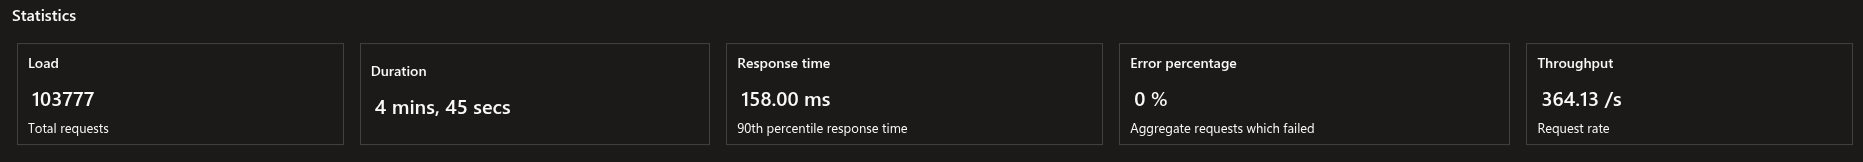
\includegraphics[width=\textwidth]{TestLettura1.png}
        \caption{158 ms su una media di 364 richieste al secondo}
    \end{center}
\end{figure}

\begin{figure}[htbp]
    \begin{center}
        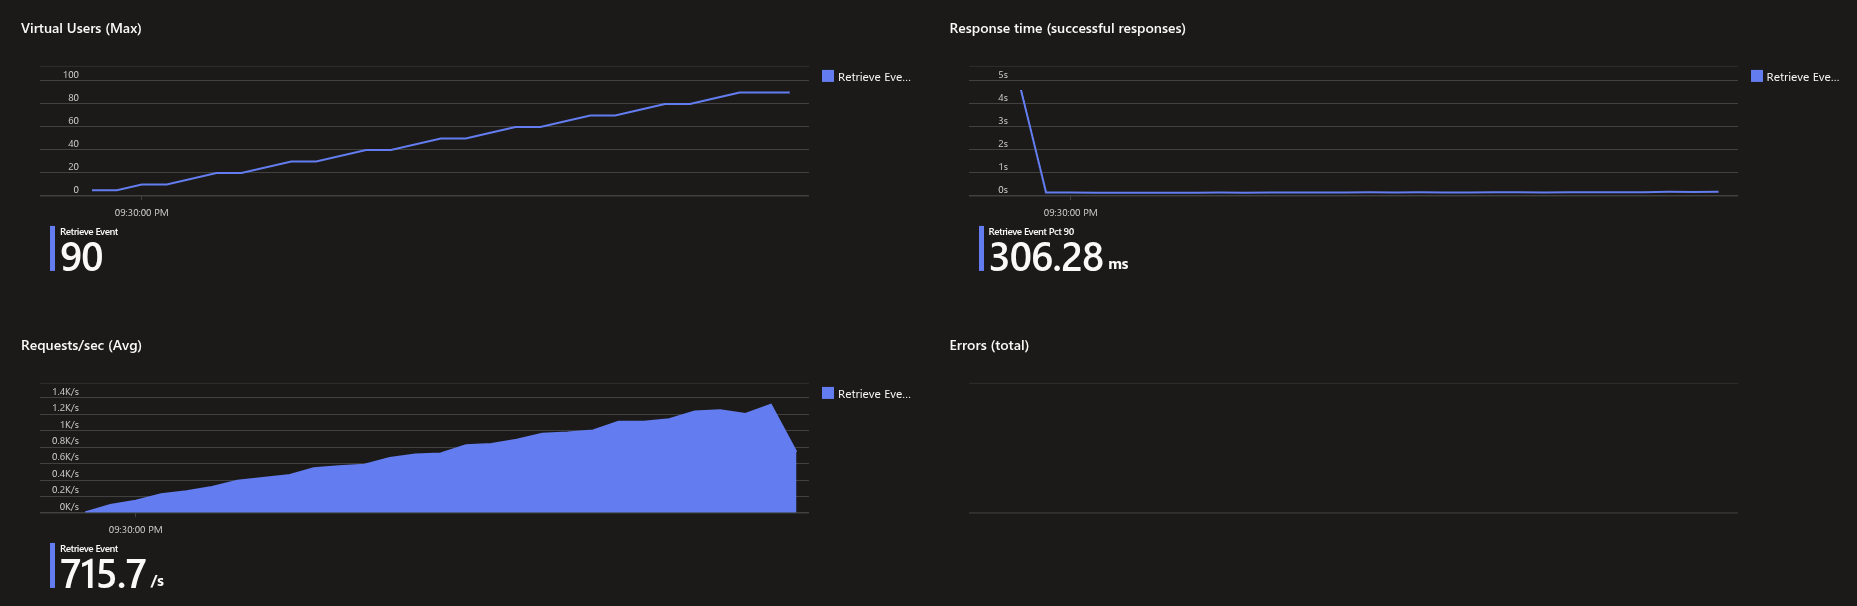
\includegraphics[width=\textwidth]{TestLettura2.png}
        \caption{il tempo di risposta non varia in base al numero di richieste}
    \end{center}
\end{figure}

\begin{figure}[htbp]
    \begin{center}
        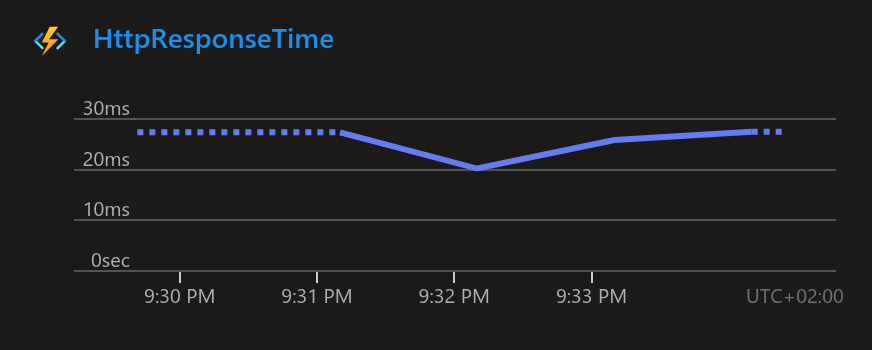
\includegraphics[width=\textwidth]{TestLettura3.png}
        \caption{Dettaglio della velocità senza tempo di trasmissione}
    \end{center}
\end{figure}
\clearpage
\section{Caricamento di immagini concorrenti}

\begin{figure}[htbp]
    \begin{center}
        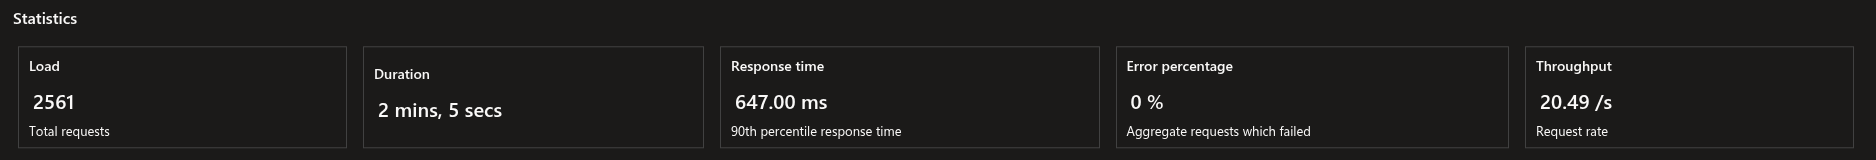
\includegraphics[width=\textwidth]{UploadImages1.png}
        \caption{2 MB di immagini in 600 ms 20 volte al secondo}  
    \end{center}
\end{figure}

\begin{figure}[htbp]
    \begin{center}
        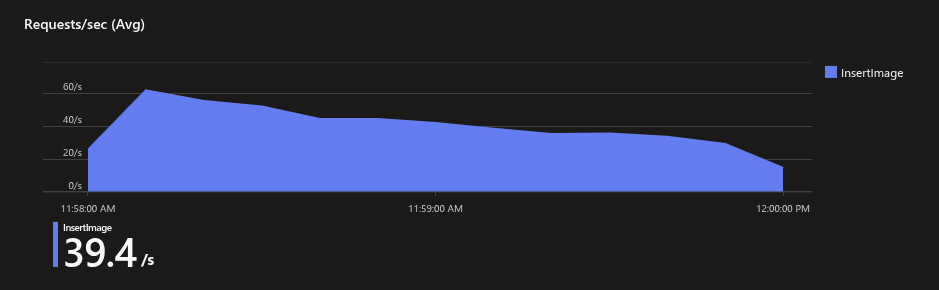
\includegraphics[width=\textwidth]{UploadImages3.png}
        \caption{Andamento delle richieste}  
    \end{center}
\end{figure}

\begin{figure}[htbp]
    \begin{center}
        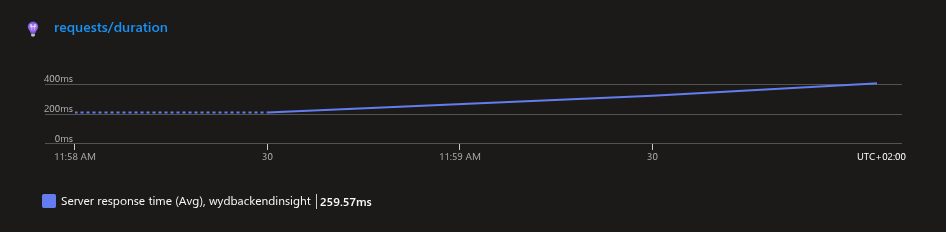
\includegraphics[width=\textwidth]{UploadImages2.png}
        \caption{Dettaglio della velocità richiesta dal server}
    \end{center}
\end{figure}


\clearpage
\chapter*{Conclusioni}
\addcontentsline{toc}{chapter}{Conclusione}

\begin{figure}[htbp]
    \begin{center}
        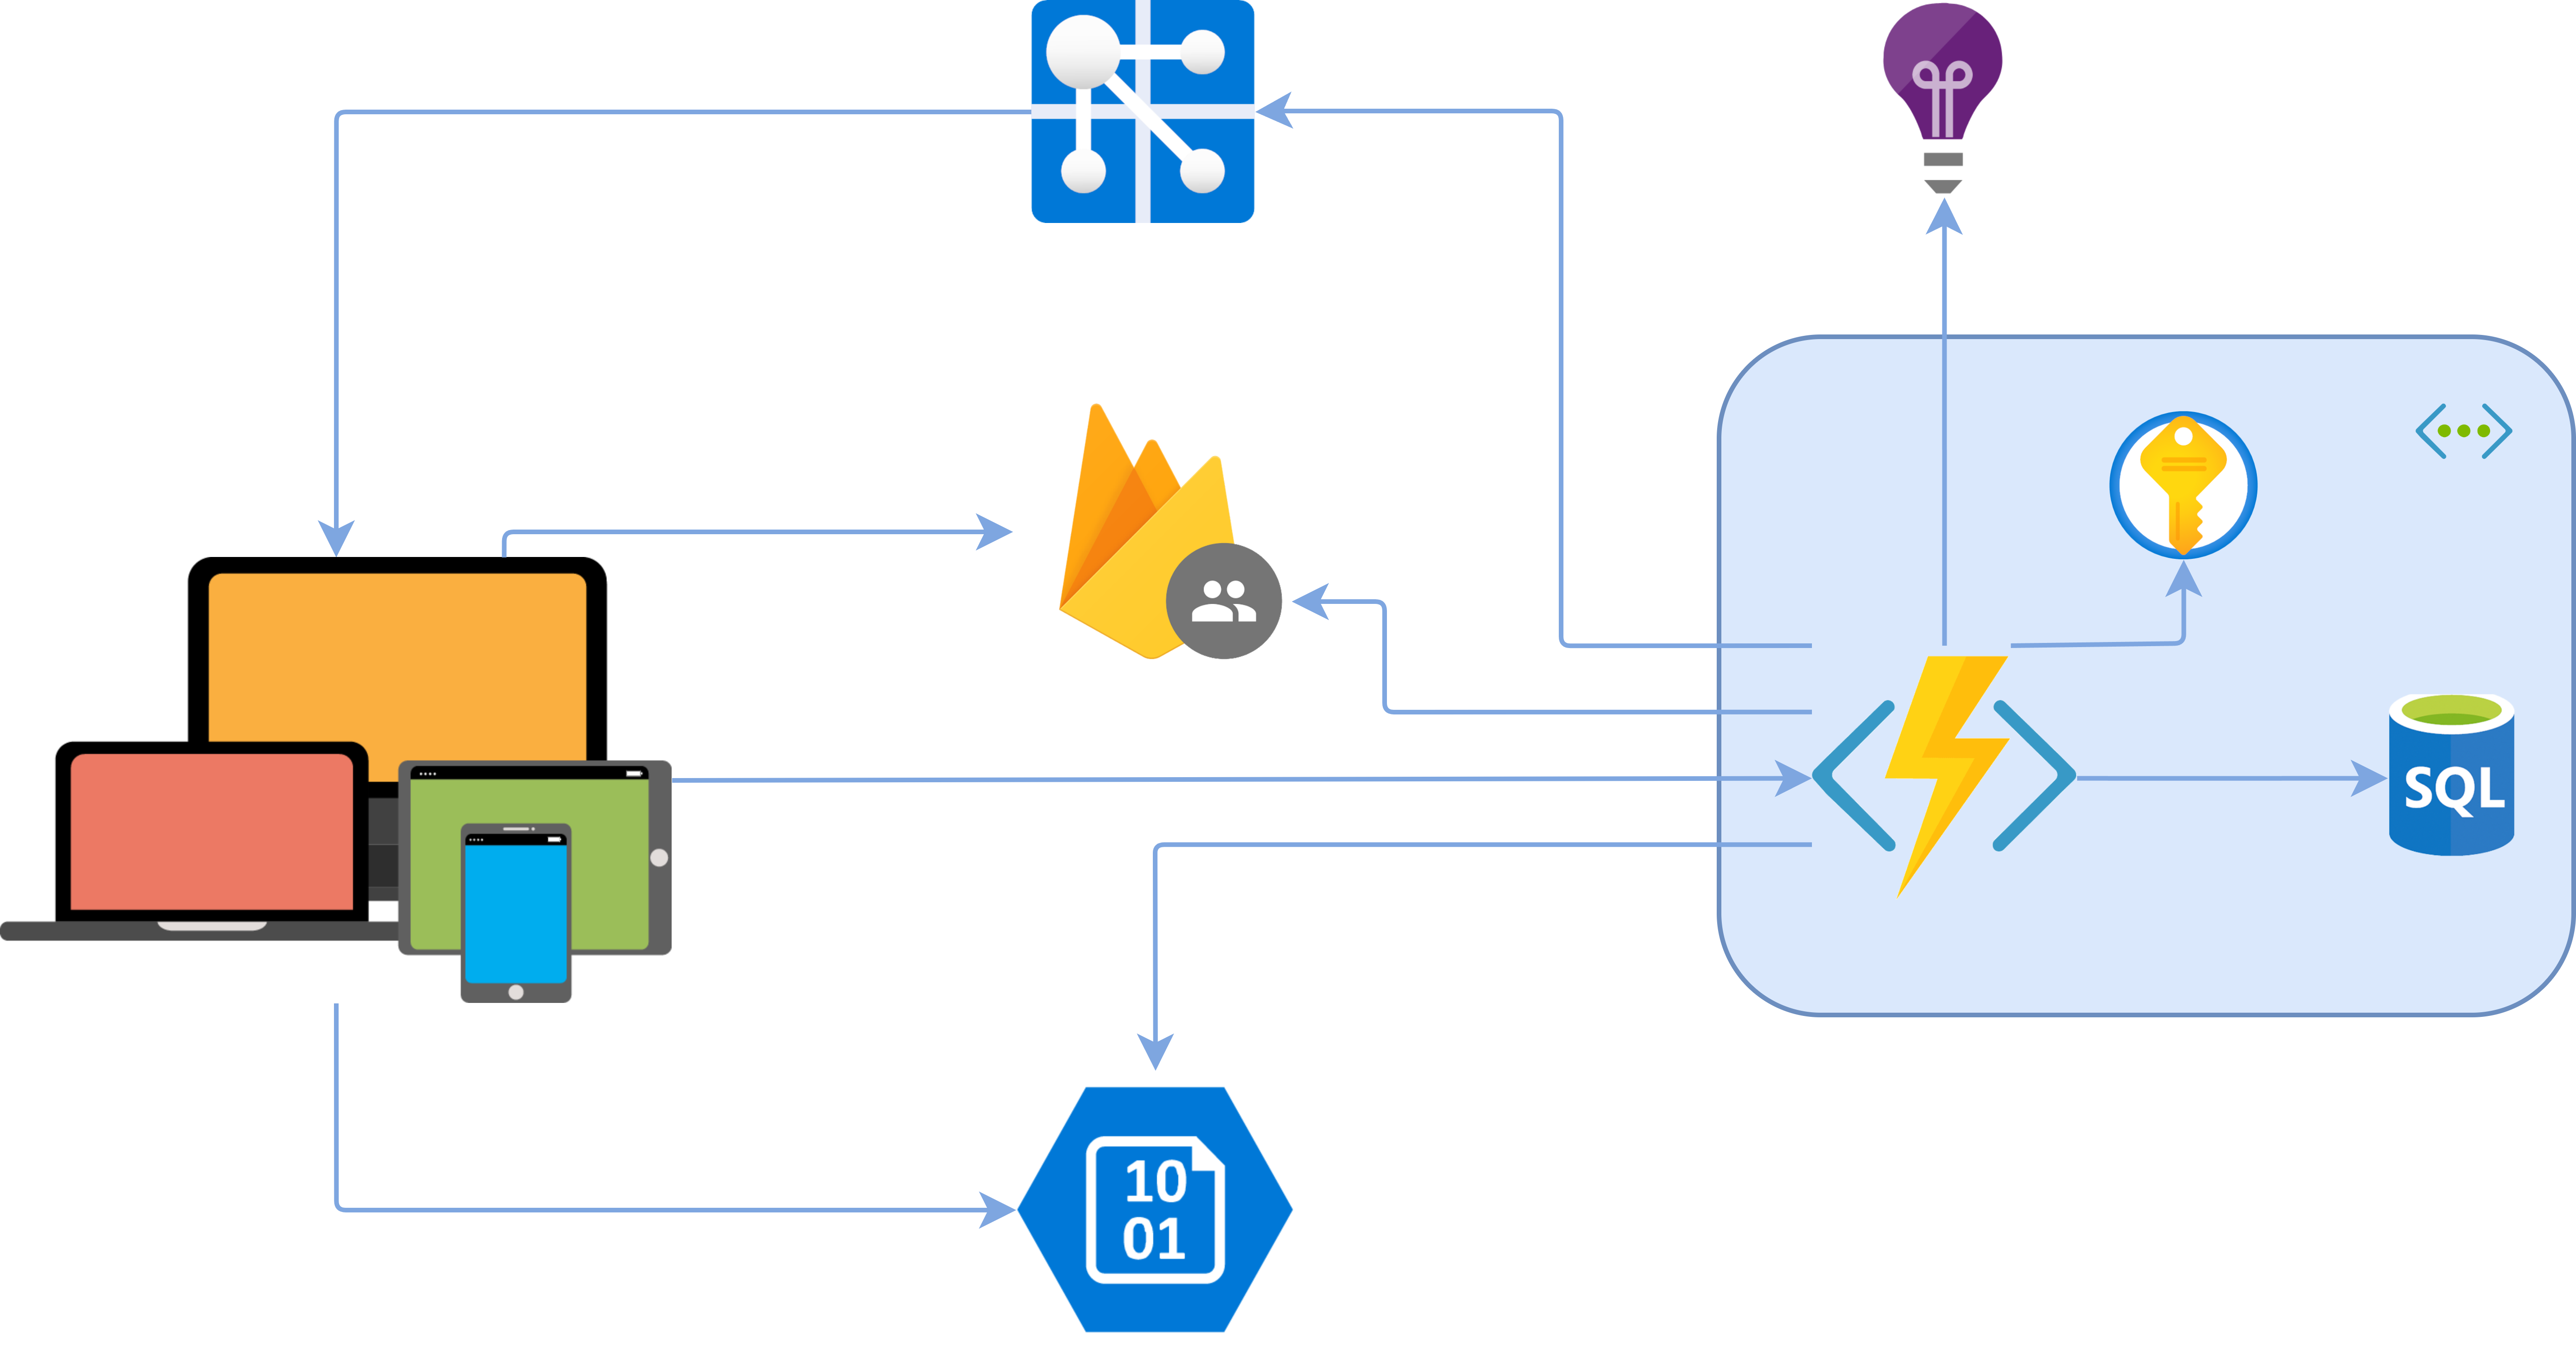
\includegraphics[width=\textwidth]{ImplementazioneArchitettura.png}
        \caption{Grafico dell'architettura di WYD}
    \end{center}
\end{figure}
\clearpage

\section{Sviluppi futuri}
Gli sviluppi futuri potranno comprendere, in base a decisioni di marketing:
\begin{itemize}
    \item La visualizzazione degli impegni degli altri profili
    \item L'implementazione di una chat per ogni gruppo
    \item Sviluppo di strumenti utili all'organizzazione dei gruppi, quali:
          \begin{itemize}
              \item form per combinare le disponibilità reciproche
              \item appunti condivisi(liste della spesa o note su chi porta cosa)
              \item calcolo delle spese compiute da ciascun componente
          \end{itemize}
    \item La creazione di profili pubblici che possono essere seguiti
    \item La creazione di eventi pubblici
    \item Una funzionalità di ricerca degli eventi o dei profili pubblici
    \item Supporto alla gestione di prenotazione e organizzazione degli eventi, dalle liste di attesa alla vendita dei biglietti
    \item La possibilità per le aziende di gestire in locale il proprio server e i relativi dati
\end{itemize}
\clearpage

\chapter*{Fonti bibliografiche e sitografia}
\addcontentsline{toc}{chapter}{Fonti bibliografiche e sitografia}

Object Management Group, OMG Unified Modelling Language Version 2.5.1, December 2017, https://www.omg.org/spec/UML/2.5.1/PDF

https://learn.microsoft.com/en-us/azure/reliability/reliability-cosmos-db-nosql
https://learn.microsoft.com/en-gb/azure/cosmos-db/throughput-serverless
https://learn.microsoft.com/en-gb/azure/cosmos-db/provision-throughput-autoscale